\section{A sharp bound from the centre and squared semiaxes}\label{sec:purity-envelope}
Let $\sigma$ be canonical, $\sigma_B=I/2$, with Alice Bloch-vector length $c$ and correlation matrix $S$. Put
\[
 Q=SS^T,\qquad q=\tr Q,\qquad P=\tr\sigma^2=\frac{1+c^2+q}{4}.
\]
Thus $q$ is the sum of the squared ellipsoid semiaxes. It requires neither their individual values nor the full signed geometry.

\begin{theorem}[Exact two-invariant envelope]\label{thm:purity-envelope}
The physically possible pairs are exactly
\[
 0\le c\le1,\qquad 0\le q\le3-4c+c^2.
\]
Among all canonical states with these invariants, the exact maximum of $\lambda_{\max}(\sigma)$ is $H(c,q)$ below.
For $0\le c\le2/3$, put $q_1=c^2/4$ and $q_2=3-6c+5c^2/2$. Then
\[
 \boxed{H(c,q)=
 \begin{cases}
 (1+c+\sqrt q)/4,&0\le q\le q_1,\\
 (1+\sqrt{3q+3c^2/2})/4,&q_1\le q\le q_2,\\
 (2-c+\sqrt{2q+4c-2-c^2})/4,&q_2\le q\le3-4c+c^2.
 \end{cases}}
\]
For $2/3\le c\le1$, the middle branch disappears:
\[
 \boxed{H(c,q)=
 \begin{cases}
 (1+c+\sqrt q)/4,&0\le q\le(1-c)^2,\\
 (2-c+\sqrt{2q+4c-2-c^2})/4,&(1-c)^2\le q\le3-4c+c^2.
 \end{cases}}
\]
Every state in the invertible Bob-filter orbit of $\sigma$ satisfies $f(\rho)\le H(c,q)$. This bound is sharp as a supremum for every allowed pair.
\end{theorem}

\subsection{Proof by exact quadratic certificates}
Write the ordered spectrum as $\lambda\ge u\ge v\ge w\ge0$, and put $h=c/2$. Bravyi's two-qubit marginal theorem~\cite{bravyi} gives
\begin{equation}\label{eq:bravyi-used}
 v+w\le\tfrac12-h,\qquad \lambda-v\ge h,\qquad u-w\ge h.
\end{equation}
The additional inequality $\lambda-w\ge h$ is redundant here. These established quantum-marginal constraints are an explicit dependency of the proof.

Trace one and the first inequality imply $\lambda\ge(1+c)/4$, while $u\ge h$ gives $\lambda\le1-h=:L$.
If $\lambda\le1/2$, then $P\le\lambda\le1/2\le L^2+(1-L)^2$.
If $\lambda\ge1/2$, then
$P\le\lambda^2+(1-\lambda)^2\le L^2+(1-L)^2$.
Hence $q\le3-4c+c^2$.

For fixed $\lambda,c$, the minimum possible purity is attained by these spectra:
\[
\begin{array}{c|c}
 \text{branch}&(\lambda,u,v,w)\\ \hline
 \mathrm I&(\lambda,\frac12-\lambda+h,\lambda-h,\frac12-\lambda)\\[2pt]
 \mathrm {II}&(\lambda,r+h/2,r,r-h/2),\quad r=(1-\lambda)/3\\[2pt]
 \mathrm {III}&(\lambda,h,1-\lambda-h,0).
\end{array}
\]
Their purities are
\begin{align*}
 P_{\mathrm I}&=\frac{1+c^2}{4}+4\left(\lambda-\frac{1+c}{4}\right)^2,\\
 P_{\mathrm {II}}&=\lambda^2+\frac{(1-\lambda)^2}{3}+\frac{c^2}{8},\\
 P_{\mathrm {III}}&=\lambda^2+h^2+(1-\lambda-h)^2.
\end{align*}
For $c\le2/3$, the branch intervals in $\lambda$ are
\[
 \left[\frac{1+c}{4},\frac{2+3c}{8}\right],\quad
 \left[\frac{2+3c}{8},1-\frac{3c}{4}\right],\quad
 \left[1-\frac{3c}{4},1-\frac c2\right].
\]
For $c\ge2/3$, branches I and III instead occupy
$[(1+c)/4,1/2]$ and $[1/2,1-c/2]$.

Here are direct certificates. If $(u_0,v_0,w_0)$ is the proposed remaining spectrum and $U=u-u_0,V=v-v_0,W=w-w_0$, then $U+V+W=0$ and
\[
 P-P_{\min}=U^2+V^2+W^2+2(u_0U+v_0V+w_0W).
\]
In branch I put $d=2\lambda-h-1/2$. The constraints imply $U\ge0$, $2U+V\ge0$, and $0\le d\le h/2$. The linear term is
\[
 u_0U+v_0V+w_0W=d(2U+V)+(h-2d)U\ge0.
\]
In branch II it is $(h/2)(U-W)\ge0$ by $u-w\ge h$.
In branch III put $v_0=1-\lambda-h$. Then $W=w\ge0$, $U-W\ge0$, and the linear term is
\[
 (h-v_0)(U-W)+(h-2v_0)W\ge0.
\]
Both coefficients are nonnegative on the stated interval. Each certificate is therefore a sum of squares and nonnegative multiples of spectral constraints. The proposed spectra satisfy ordering and all constraints. Their purities increase with $\lambda$, agree at the joins, and inversion gives $H$.

\subsection{Sharp states}
For each optimizing spectrum, $u-w=h$. Define
\[
 a=\frac{\lambda+v+h}{2},\qquad d=\frac{\lambda+v-h}{2},\qquad
 z=\frac{\sqrt{(\lambda-v)^2-h^2}}2,
\qquad
 \sigma=\begin{pmatrix}
 a&0&0&z\\0&u&0&0\\0&0&w&0\\z&0&0&d
 \end{pmatrix}.
\]
The correlated block has eigenvalues $\lambda,v$, the other eigenvalues are $u,w$, and the marginals are $\diag((1+c)/2,(1-c)/2)$ and $I/2$. This realizes every allowed pair and proves sharpness. No converse invocation of Bravyi is needed.

The supremum of FEF in a canonical state's invertible Bob-filter orbit is its top eigenvalue, as established in Section~\ref{sec:shape}. In the interiors of branches II and III, $z>0$ and the top eigenvector is entangled, so an invertible filter attains $H$. Product top eigenvectors can be approached by invertible filters, proving sharpness as a supremum elsewhere. Singular output limits require recomputing the ellipsoid; point ellipsoids can persist at such a limit.

\paragraph{An exact strict improvement.}
At $c=3/5,q=2/5$,
\[
 H(c,q)=\frac{7+\sqrt{21}}{20}\simeq0.57913<\frac7{10}.
\]
An attaining canonical state is
\[
 \sigma=\begin{pmatrix}
 1/2&0&0&\sqrt3/10\\
 0&3/10&0&0\\
 0&0&0&0\\
 \sqrt3/10&0&0&1/5
 \end{pmatrix}.
\]
For $b=3/\sqrt{21}$ and $K=\diag(\sqrt{1+b},\sqrt{1-b})$, the normalized state $(I\otimes K)\sigma(I\otimes K)$ has Bell overlap
\[
 \frac7{20}+\frac{3b}{20}+\frac{\sqrt3}{10}\sqrt{1-b^2}
       =\frac{7+\sqrt{21}}{20}.
\]
The filter preserves the ellipsoid, so this is actual FEF attainment.

\begin{figure}[htbp]\centering
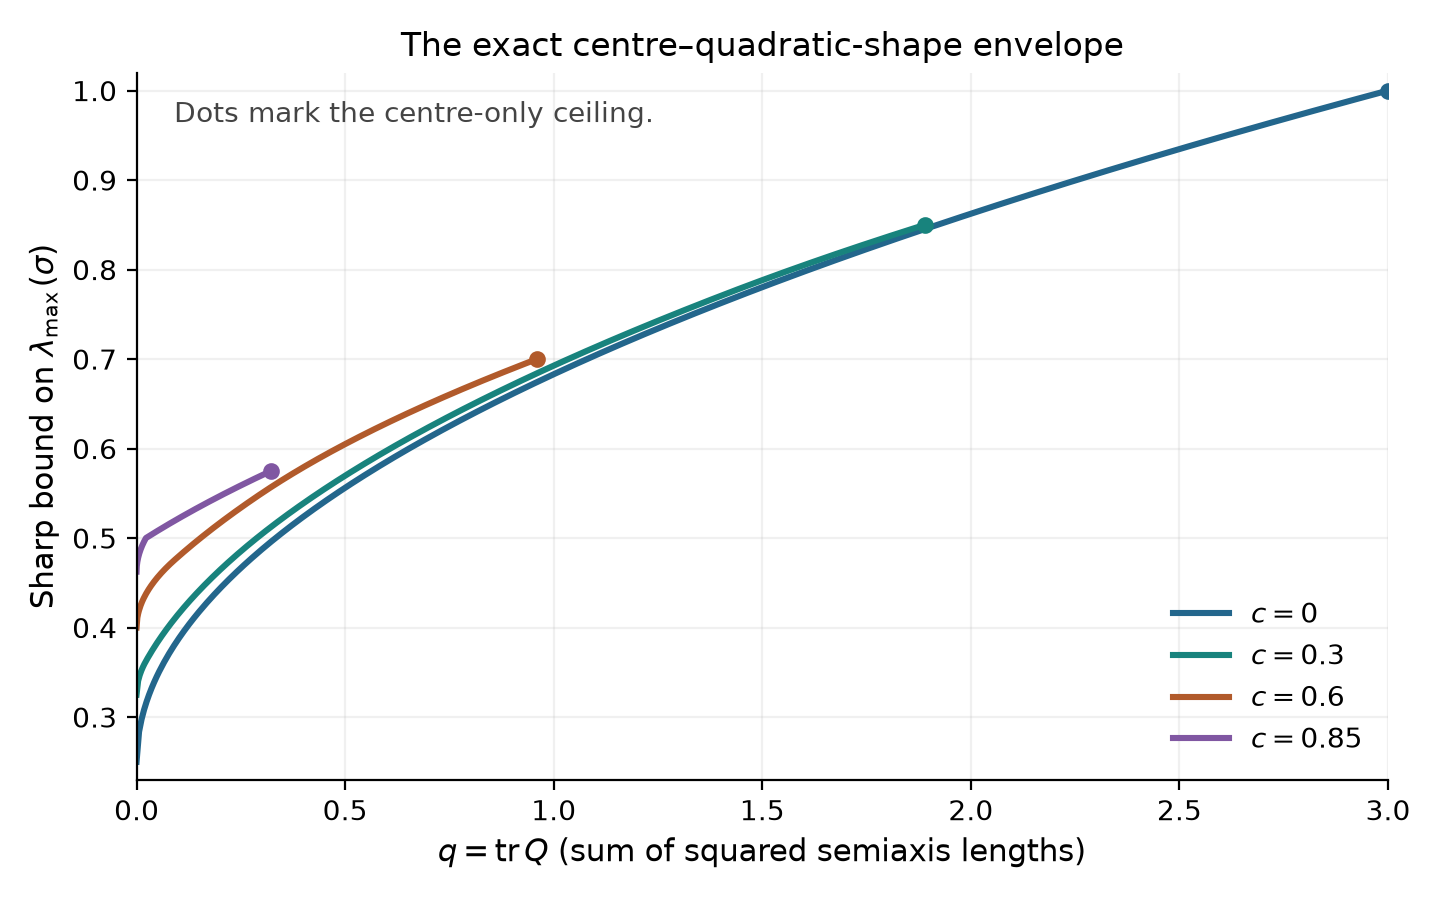
\includegraphics[width=.96\textwidth]{purity_envelope.png}
\caption{The exact two-invariant envelope. The analytic branches meet continuously; the centre-only bound is recovered at the largest allowed $q$. Curves evaluate the proved formulas.}
\end{figure}
